\documentclass{article}
\usepackage{tikz}
\usetikzlibrary{calc,scopes}

\begin{document}

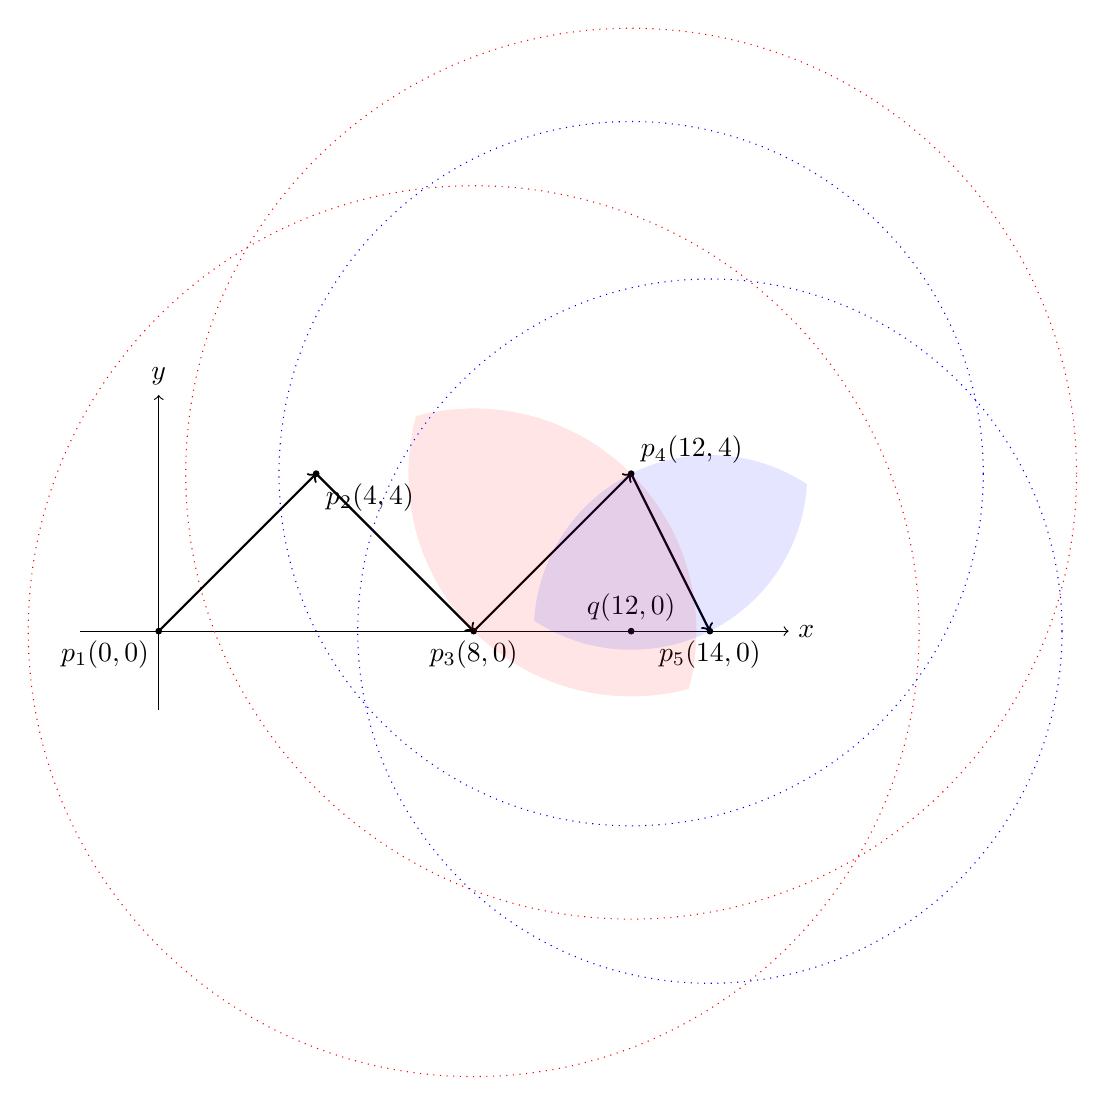
\begin{tikzpicture}[scale=0.5]
    % Define coordinates
    \coordinate (p1) at (0,0);
    \coordinate (p2) at (4,4);
    \coordinate (p3) at (8,0);
    \coordinate (p4) at (12,4);
    \coordinate (p5) at (14,0);
    \coordinate (q) at (12,0);

    % Draw axes
    \draw[->] (-2,0) -- (16,0) node[right] {$x$};
    \draw[->] (0,-2) -- (0,6) node[above] {$y$};

    % Draw points
    \filldraw (p1) circle (2pt) node[below left] {$p_1(0,0)$};
    \filldraw (p2) circle (2pt) node[below right] {$p_2(4,4)$};
    \filldraw (p3) circle (2pt) node[below] {$p_3(8,0)$};
    \filldraw (p4) circle (2pt) node[above right] {$p_4(12,4)$};
    \filldraw (p5) circle (2pt) node[below] {$p_5(14,0)$};
    \filldraw (q) circle (2pt) node[above] {$q(12,0)$};

    % Draw directed edges
    \draw[->, thick] (p1) -- (p2);
    \draw[->, thick] (p2) -- (p3);
    \draw[->, thick] (p3) -- (p4);
    \draw[->, thick] (p4) -- (p5);

    % Lune for (p3, p4)
    \path let \p1=(p3), \p2=(p4), \n1={veclen(\x2-\x1,\y2-\y1)} in
        node[draw, circle, red, dotted, minimum size=2*\n1] at (\p1) {}
        node[draw, circle, red, dotted, minimum size=2*\n1] at (\p2) {};

    \begin{scope}
        \clip let \p1=(p3), \p2=(p4), \n1={veclen(\x2-\x1,\y2-\y1)} in
            (p3) circle (\n1);
        \path let \p1=(p3), \p2=(p4), \n1={veclen(\x2-\x1,\y2-\y1)} in
            (p4) circle (\n1) [fill=red, fill opacity=0.1];
    \end{scope}

    % Lune for (p4, p5)
    \path let \p1=(p4), \p2=(p5), \n1={veclen(\x2-\x1,\y2-\y1)} in
        node[draw, circle, blue, dotted, minimum size=2*\n1] at (\p1) {}
        node[draw, circle, blue, dotted, minimum size=2*\n1] at (\p2) {};

    \begin{scope}
        \clip let \p1=(p4), \p2=(p5), \n1={veclen(\x2-\x1,\y2-\y1)} in
            (p4) circle (\n1);
        \path let \p1=(p4), \p2=(p5), \n1={veclen(\x2-\x1,\y2-\y1)} in
            (p5) circle (\n1) [fill=blue, fill opacity=0.1];
    \end{scope}

\end{tikzpicture}

\end{document}
